\documentclass[a4paper, 12pt]{article}
\usepackage[UTF8]{ctex}
\usepackage{amsmath, amssymb}
\usepackage{graphicx}
\usepackage{float}
\usepackage{geometry}
\usepackage{booktabs}
\usepackage{hyperref}
\usepackage{xcolor}
\usepackage{listings}
\usepackage{caption}
\usepackage{subcaption}
\usepackage{enumitem}
\usepackage{array}

\newcommand{\placeholderfigure}[2]{
    \begin{figure}[H]
        \centering
        \fbox{
            \begin{minipage}[c][0.25\textheight][c]{0.8\linewidth}
                \centering
                #1
            \end{minipage}
        }
        \caption{#2}
    \end{figure}
}

\geometry{left=2.5cm, right=2.5cm, top=2.5cm, bottom=2.5cm}

\hypersetup{
    colorlinks=true,
    linkcolor=blue!70!black,
    citecolor=green!50!black,
    urlcolor=blue!60!black
}

\lstset{
    language=Python,
    basicstyle=\ttfamily\small,
    keywordstyle=\color{blue}\bfseries,
    commentstyle=\color{green!50!black}\itshape,
    stringstyle=\color{red!70!black},
    numbers=left,
    numberstyle=\tiny\color{gray},
    frame=single,
    breaklines=true,
    tabsize=4,
    captionpos=b
}

\title{\textbf{县域乡镇村巡视路线优化建模} \\ \large 基于图距离闭包、候选路线审计与参数敏感性分析的建模报告}
\author{林欣志 \quad 汪伯治}
\date{\today}

\begin{document}

\maketitle

\begin{abstract}
本文研究某县洪灾后乡镇村巡视路线规划问题。
道路网络被建模为无向加权图，边权表示道路里程。
所有巡视路线均从县政府所在地 $O$ 出发，并最终返回 $O$。
乡镇节点和村节点是必须巡视的服务点，辅助道路节点只参与通行路径。

本文从图论和数学规划角度建立统一模型，给出距离闭包、路线耗时、组数下界和参数敏感性分析方法。
汪伯治负责路线构造与优化算法，林欣志负责耗时审计、下界分析、参数分析和交互式可视化。
文中数值由正式道路网络和候选路线复算得到。
\end{abstract}

\tableofcontents
\newpage

%==========================================================================
\section{问题说明}
%==========================================================================

某年夏天，该县遭受水灾。
县领导需要带领有关部门负责人从县政府所在地出发，对全县各乡镇和村进行巡视。
题面给出一张县域公路网，路段权重表示公里数。
巡视人员可以分为若干组同时行动。
每一组从节点 $O$ 出发，访问分配给该组的乡镇和村，然后回到 $O$。

题目包含四个要求：
\begin{enumerate}[leftmargin=2em]
    \item 固定 $3$ 组巡视，设计总路程较短且各组负载较均衡的路线；
    \item 在 $T=2\text{h}$、$t=1\text{h}$、$v=35\text{km/h}$、$24\text{h}$ 限制下，求至少需要的组数；
    \item 当巡视人员足够多时，求最短完成时间及对应路线；
    \item 固定组数时，讨论 $T$、$t$、$v$ 改变对路线选择和完成时间的影响。
\end{enumerate}

图~\ref{fig:road-network-source} 给出了报告使用的路网布局。
该布局只用于可视化。
所有距离计算仍以道路表中的边权和最短路为准。

\begin{figure}[H]
    \centering
    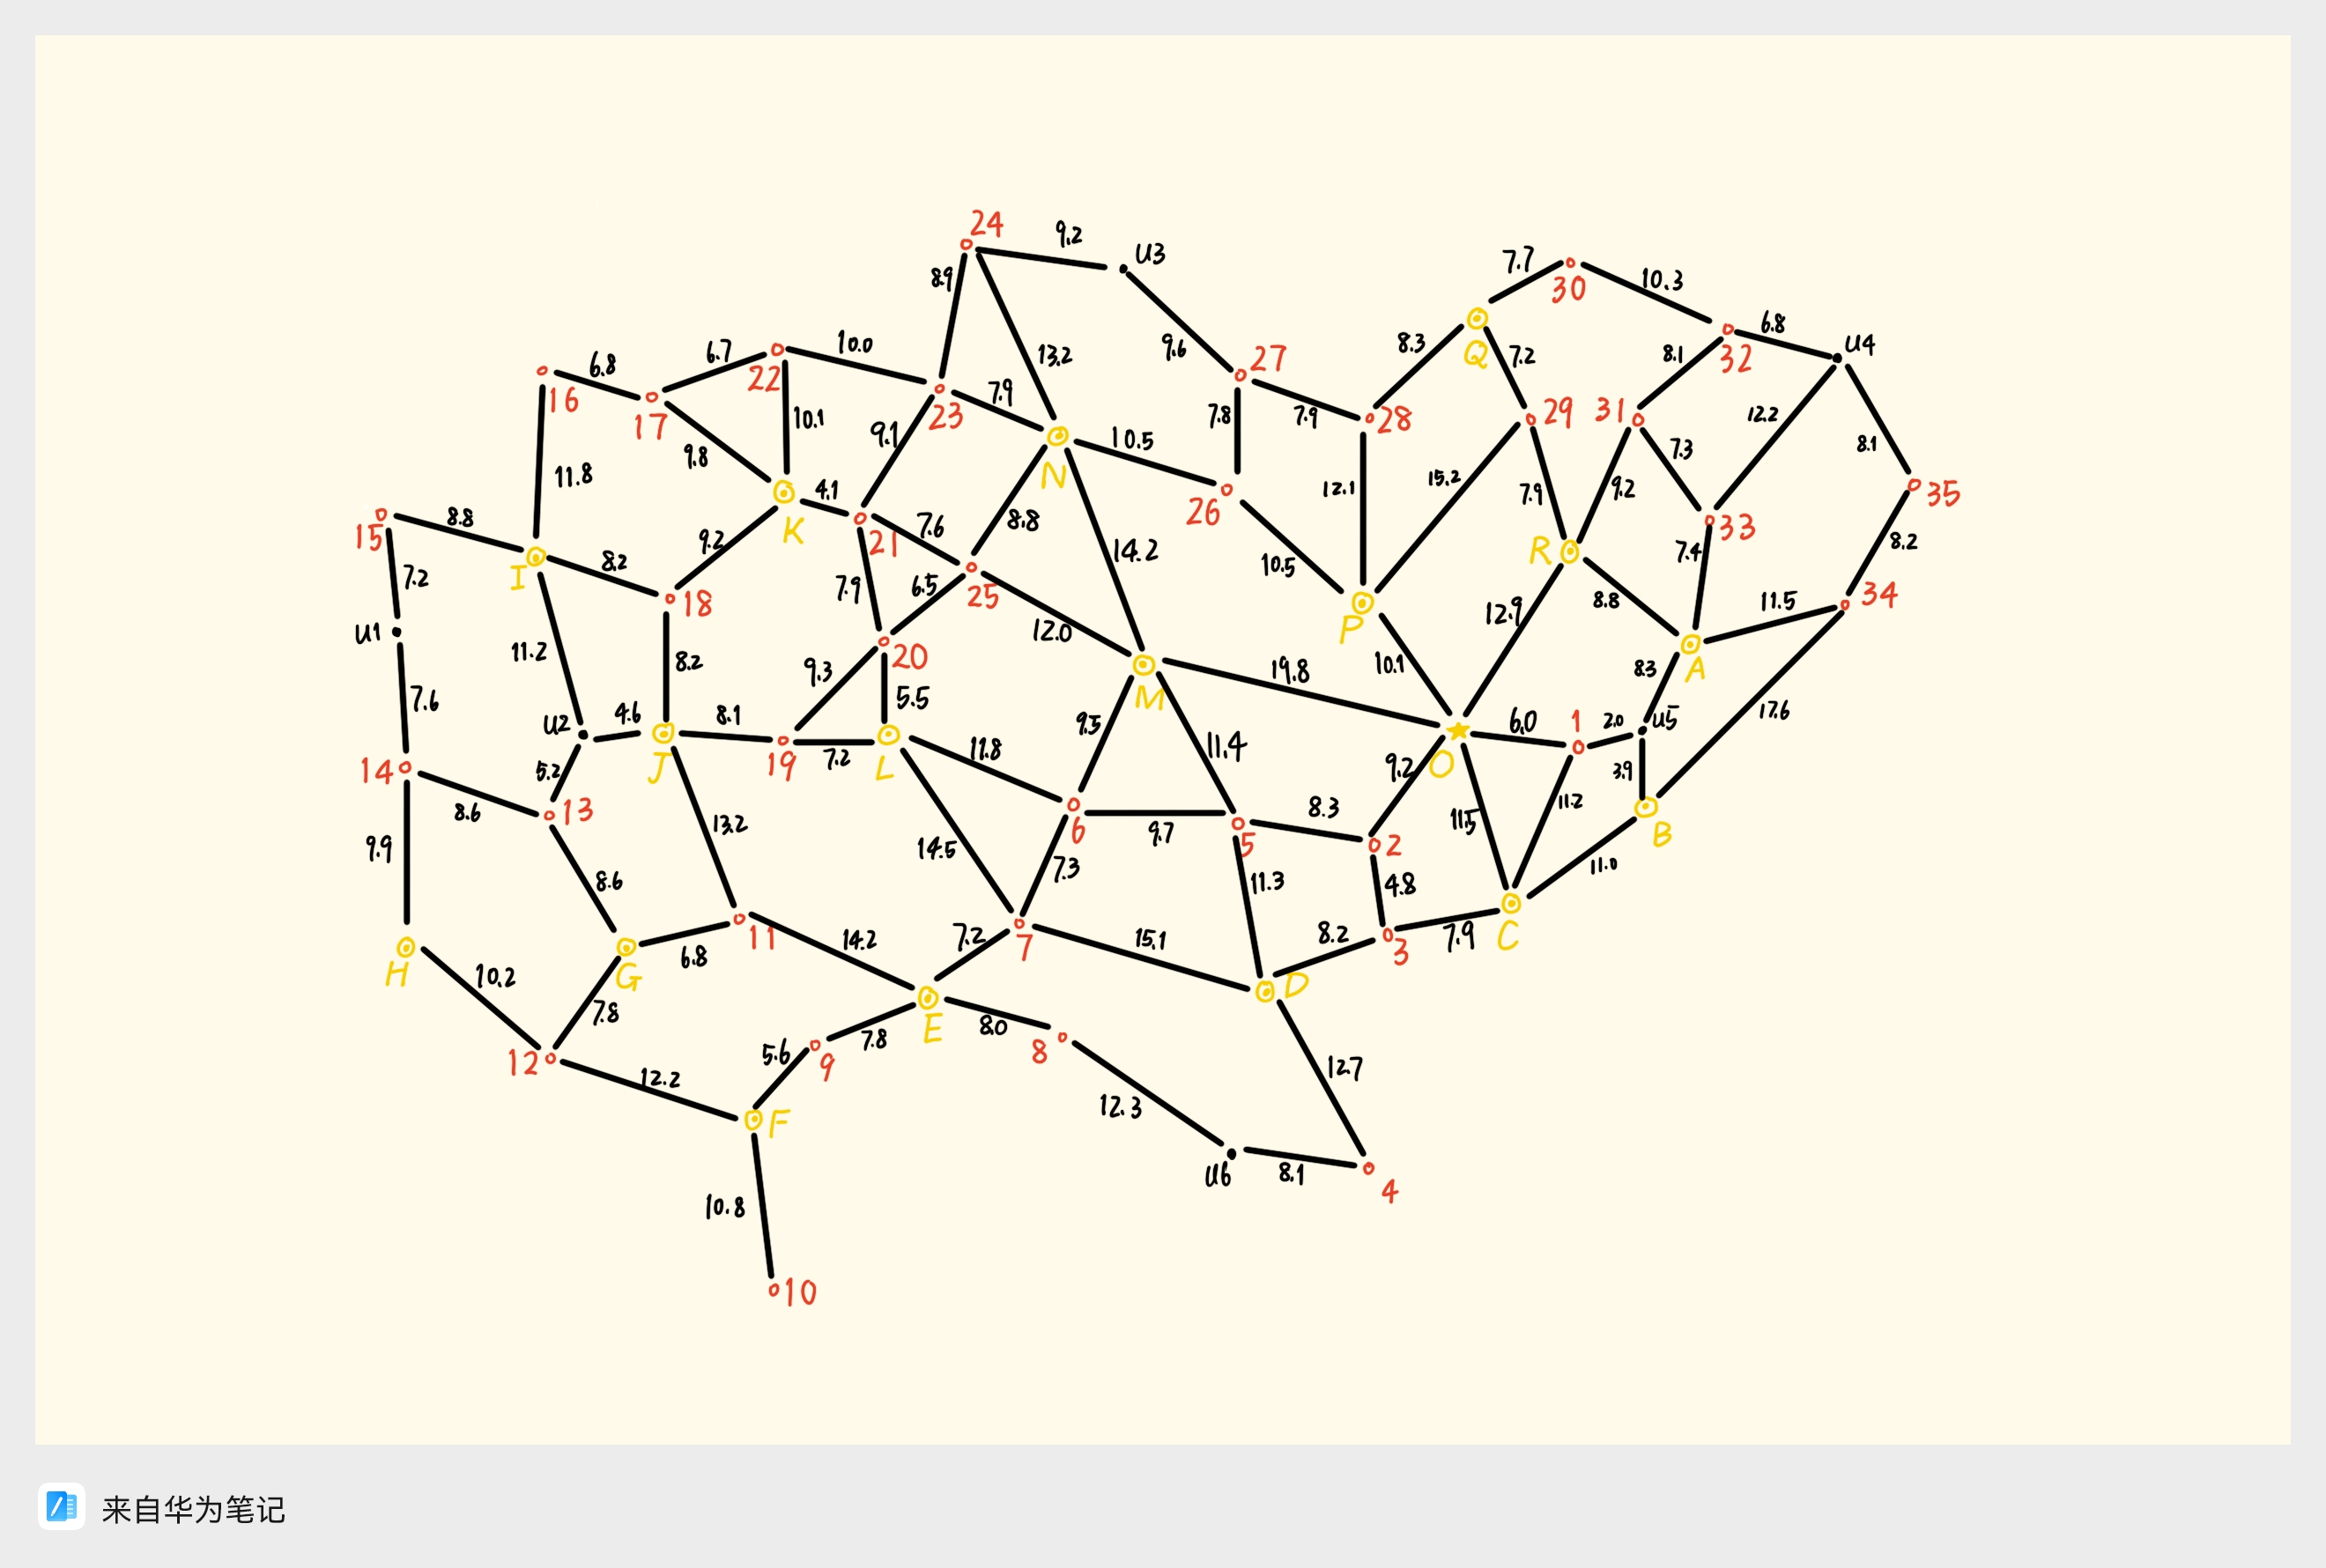
\includegraphics[width=0.92\linewidth]{figures/road_network_source.png}
    \caption{县域道路网络直线转录图。字母节点表示乡镇，数字节点表示村，$O$ 为县政府所在地。}
    \label{fig:road-network-source}
\end{figure}

本项目采用如下节点语义：
\begin{itemize}[leftmargin=2em]
    \item $O$：县政府所在地，作为所有路线的出发点和返回点；
    \item $A$--$R$ 中除 $O$ 外的字母节点：乡镇节点，共 $17$ 个；
    \item $1$--$35$：村节点，共 $35$ 个；
    \item $U1$--$U6$：辅助道路节点，共 $6$ 个，只用于保留道路拓扑和路段权重。
\end{itemize}

正式路网共有 $59$ 个节点和 $94$ 条无向边。
必须巡视的服务点共有 $52$ 个。

%==========================================================================
\section{基本假设与符号约定}
%==========================================================================

设道路网络为无向加权图
\begin{equation}
    G=(V,E,w),
\end{equation}
其中 $V$ 是节点集合，$E$ 是道路集合，$w(e)>0$ 是道路 $e$ 的长度，单位为公里。
记县政府所在地为 $O$。
乡镇节点集合为 $V_T$，村节点集合为 $V_C$，辅助道路节点集合为 $V_U$。
必须巡视的节点集合为
\begin{equation}
    R = V_T \cup V_C.
\end{equation}

对任意两个节点 $i,j\in V$，记 $d(i,j)$ 为它们在原始道路网络 $G$ 上的最短路距离。
该距离允许经过辅助道路节点。
辅助道路节点不产生停留时间，也不进入必须巡视顺序。

一条巡视路线记为
\begin{equation}
    \pi_r = (q_{r,1},q_{r,2},\ldots,q_{r,n_r}),\qquad q_{r,i}\in R.
\end{equation}
其含义是第 $r$ 组依次巡视这些乡镇或村。
车辆的实际通行路径由相邻服务点之间的最短路拼接得到，首尾补入 $O$。

路线 $\pi_r$ 的行驶距离为
\begin{equation}
    D_r =
    d(O,q_{r,1})
    + \sum_{i=1}^{n_r-1} d(q_{r,i},q_{r,i+1})
    + d(q_{r,n_r},O).
    \label{eq:route-distance}
\end{equation}
若该路线中乡镇节点数为 $a_r$，村节点数为 $b_r$，则总耗时为
\begin{equation}
    C_r = \frac{D_r}{v} + a_r T + b_r t.
    \label{eq:route-time}
\end{equation}
全方案完成时间取所有路线中耗时的最大值：
\begin{equation}
    C = \max_r C_r.
    \label{eq:completion-time}
\end{equation}
总路程为 $\sum_r D_r$。
均衡性主要用路线距离极差和路线耗时极差描述：
\begin{equation}
    \Delta_D=\max_r D_r-\min_r D_r,\qquad
    \Delta_C=\max_r C_r-\min_r C_r.
\end{equation}

%==========================================================================
\section{建模过程}
%==========================================================================

\subsection{从道路表到图模型}

数学建模的一般过程强调先抽象对象、变量和约束，再建立可计算模型并解释结果~\cite{tan2019}。
原始题面包含道路端点和路段长度。
为了避免不同模块对节点语义产生偏差，项目把道路表固化为
\texttt{data/raw/road\_network.tsv}。
读取阶段检查表头、边权正值、重复无向边、未知节点、必访节点覆盖和整图连通性。
这一步保证后续算法面对的是同一张图。

图论理论为本题提供了自然语言。
道路是边，乡镇村和交叉点是点。
参考扫雪问题中的欧拉图思想，路线规划的关键在于图结构、闭合路线、重复路程和负载均衡。
本题的目标经过进一步辨析后落在“访问所有服务点”上。
因此，本文采用必访节点上的最短路闭包建模。
欧拉图思想作为背景解释和拓展讨论，核心计算使用公式~\eqref{eq:route-distance}--\eqref{eq:completion-time}。

\subsection{必访顺序与实际路径分离}

一条路线同时包含两个层次：
\begin{itemize}[leftmargin=2em]
    \item \textbf{必访顺序}：真正需要停留和服务的乡镇、村节点；
    \item \textbf{实际通行路径}：车辆在道路网络中真实经过的节点序列。
\end{itemize}

这种分离很重要。
例如，车辆从 $O$ 到某个村可能经过 $U5$。
该辅助节点只说明道路走法，不会产生巡视任务。
正式方案只把乡镇和村写入必访顺序，实际通行路径在审计和可视化阶段由最短路展开。

\subsection{路线方案的统一表达}

为保证路线构造、耗时复算和结果展示使用同一套口径，本文采用统一的路线方案表达。
一个方案包含：
\begin{itemize}[leftmargin=2em]
    \item 方案编号、来源和参数；
    \item 若干条路线，每条路线给出路线编号、出发点和必访节点顺序；
    \item 可选的展开路径、距离和复算指标；
    \item 全方案指标和审计结果。
\end{itemize}

其核心约束如下：
\begin{enumerate}[leftmargin=2em]
    \item \texttt{depot} 固定为 $O$；
    \item \texttt{required\_visit\_order} 不写 $O$；
    \item \texttt{required\_visit\_order} 不写 $U1$--$U6$；
    \item 所有乡镇和村在正式方案中应恰好覆盖一次；
    \item 距离和耗时以复算结果为准。
\end{enumerate}

\subsection{四个问题的统一目标}

第 (1) 问固定 $k=3$。
本文把它表达为多目标排序问题：
\begin{equation}
    \min \left(
    \sum_{r=1}^{3} D_r,\;
    \Delta_D,\;
    \max_r D_r
    \right).
    \label{eq:problem-one}
\end{equation}
总路程优先，均衡指标作为次级准则。

第 (2) 问寻找最小组数：
\begin{equation}
    \min k,\qquad \text{s.t.}\quad C(k)\le 24.
    \label{eq:problem-two}
\end{equation}
一旦找到可行 $k$，还需结合下界排除更小组数。

第 (3) 问允许人员足够多。
在这种设定下，每个必访点都可以被单独安排一条路线。
对任意节点 $q\in R$，至少有一组人员从 $O$ 到达 $q$ 并返回 $O$，因此有下界
\begin{equation}
    C^\star \ge
    \max_{q\in R}
    \left(
        \frac{2d(O,q)}{v}+s(q)
    \right),
    \label{eq:single-node-lower-bound}
\end{equation}
其中 $s(q)=T$ 表示乡镇停留时间，$s(q)=t$ 表示村停留时间。
单点一组方案可以达到这个下界，因此它给出可证明的最短完成时间。

第 (4) 问固定组数并改变参数。
对每个参数情景
\begin{equation}
    \theta=(T,t,v),
\end{equation}
重新计算所有候选方案的 $C_r(\theta)$、$C(\theta)$、瓶颈路线和负载分解。
当候选赢家、瓶颈路线或耗时极差发生明显变化时，给出重新优化提示。

%==========================================================================
\section{算法原理}
%==========================================================================

\subsection{距离闭包}

直接在原始道路网络上搜索多路线方案会反复调用最短路。
本项目先在必访节点与 $O$ 之间构造距离闭包。
设
\begin{equation}
    \bar{V}=R\cup\{O\}.
\end{equation}
对 $\bar{V}$ 中任意两个节点 $i,j$，保存最短距离 $d(i,j)$ 和对应节点路径。
之后的路线评分只需查表。
导出正式路线或播放动画时，再把相邻必访点之间的最短路展开为原始道路节点序列。

\subsection{候选解评分}

路线构造程序内部使用候选解
\begin{equation}
    X=(\pi_1,\pi_2,\ldots,\pi_k).
\end{equation}
评分函数根据目标设置输出总距离、最大路线距离、距离极差、总耗时、最大路线耗时、耗时极差和惩罚项。
惩罚项用于处理缺失节点、重复节点、空路线、组数不匹配和超时。
正式结果只展示通过最终审计的方案。

\subsection{路线构造算法}

\subsection{优化算法}

\placeholderfigure{此处放置最终路线构造算法流程图。建议展示：距离闭包、初始构造、局部搜索、方案池保留、统一路线方案和最终审计。}{路线构造算法流程图占位}

%==========================================================================
\section{审计、下界与参数分析}
%==========================================================================

\subsection{耗时评价器}

评价器对任意路线方案复算距离和耗时。
它只根据必访顺序和道路网络最短路计算指标，不信任输入文件自带的距离字段。
对第 $r$ 条路线，评价器输出：
\begin{equation}
\begin{aligned}
    D_r &= \text{route distance},\\
    T^{\text{travel}}_r &= D_r/v,\\
    T^{\text{town}}_r &= a_rT,\\
    T^{\text{village}}_r &= b_rt,\\
    C_r &= T^{\text{travel}}_r+T^{\text{town}}_r+T^{\text{village}}_r.
\end{aligned}
\end{equation}

全方案输出总路程、最长路线距离、最短路线距离、距离极差、完成时间和耗时极差。
这些指标用于路线比较、可行性判断和后续路线优化。

\subsection{可行性审计}

审计器在评价器之上判断方案是否可进入正式结果讨论。
审计结果分为四类：
\begin{itemize}[leftmargin=2em]
    \item \textbf{schema valid}：字段和契约版本正确；
    \item \textbf{coverage valid}：所有必访节点覆盖一次；
    \item \textbf{route valid}：路线首尾、展开路径和节点语义合法；
    \item \textbf{metric valid}：输入指标与复算指标一致。
\end{itemize}

审计器提供候选模式和最终模式。
候选模式用于定位中间方案问题。
最终模式用于报告和正式展示。
报告结论只使用最终模式通过的方案。

\subsection{组数下界}

第 (2) 问的最小组数需要同时使用候选上界和数学下界。
一个直接而严格的下界来自总停留时间。
所有乡镇和村必须被服务一次，因此总停留时间为
\begin{equation}
    L_{\text{stop}}=|V_T|T+|V_C|t.
\end{equation}
在题面默认参数下，
\begin{equation}
    L_{\text{stop}}=17\times2+35\times1=69\text{h}.
\end{equation}
若有 $k$ 组并行巡视，则完成时间至少为
\begin{equation}
    C\ge \frac{69}{k}.
\end{equation}
因此 $k=1$ 和 $k=2$ 均无法在 $24$ 小时内完成。
图~\ref{fig:lower-bound-by-group} 展示了 $k=1$ 到 $8$ 的严格下界。

\begin{figure}[H]
    \centering
    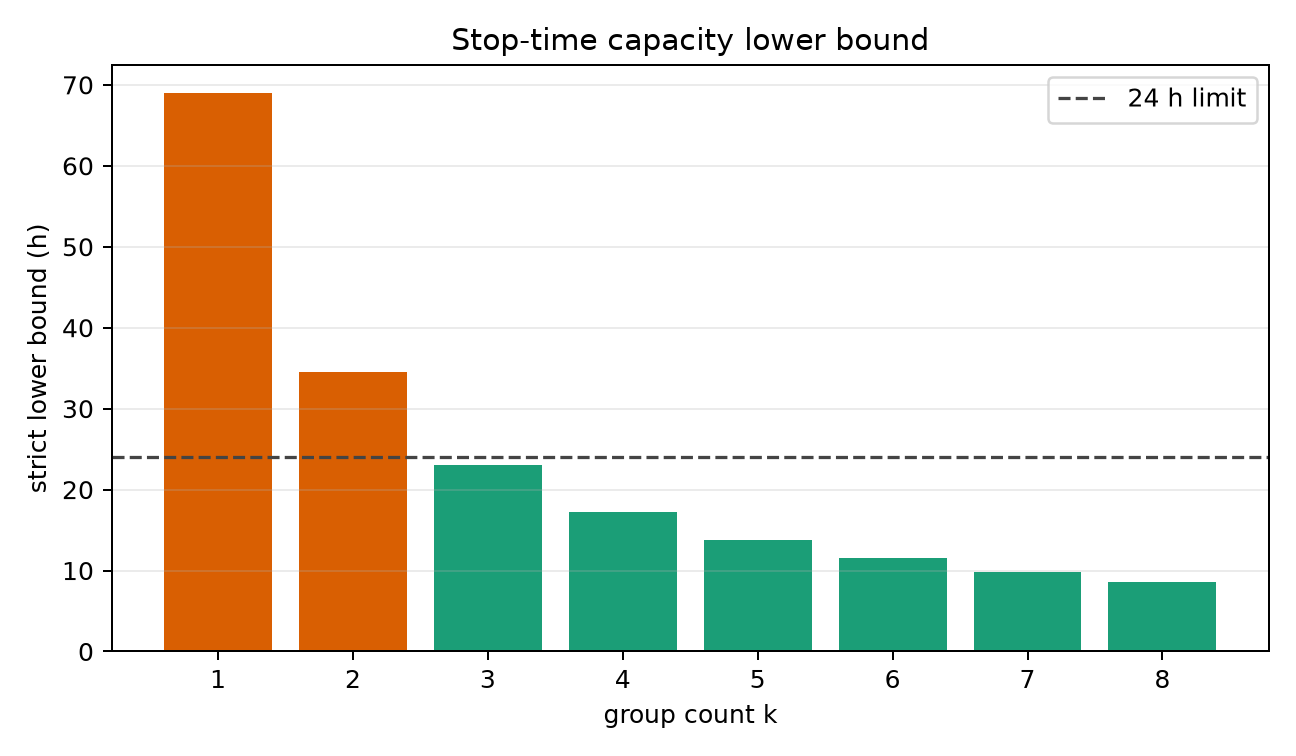
\includegraphics[width=0.78\linewidth]{figures/lower_bound_by_group.png}
    \caption{停留时间容量下界。虚线为 $24$ 小时限制。}
    \label{fig:lower-bound-by-group}
\end{figure}

在当前默认参数下，停留时间下界只能排除 $1$ 组和 $2$ 组。
要证明某个更大的组数是否最少，还需要候选路线达到 $24$ 小时限制，并结合更强下界或完备搜索信息。

\subsection{人员足够时的最短完成时间}

第 (3) 问使用公式~\eqref{eq:single-node-lower-bound}。
当前路网中产生最大单点往返下界的节点是 $H$。
在 $T=2\text{h}$、$t=1\text{h}$、$v=35\text{km/h}$ 下，该下界为
\begin{equation}
    6.428571\text{h}.
\end{equation}
单点一组构造能够达到该值。
所以人员足够时，最短完成时间可被证明为约 $6.43$ 小时。
后续路线构造部分可以在保持该最短时间的前提下，进一步比较组数、总路程和均衡性。

\subsection{参数敏感性分析}

参数敏感性分析接收一批代表性候选方案。
它不在内部重新搜索路线。
对每个情景，它执行最终审计、复算指标、排序候选，并记录瓶颈路线和耗时分解。

默认代表性情景包括：
\begin{equation}
    T\in\{1.5,2.0,2.5\},\quad
    t\in\{0.5,1.0,1.5\},\quad
    v\in\{25,35,45\},
\end{equation}
并以 $(2,1,35)$ 为基准。
当完成时间相对基准增加超过 $10\%$、瓶颈路线切换、候选赢家变化或耗时极差超过阈值时，报告给出重新优化提示。

图~\ref{fig:sensitivity-completion-time} 展示了同一路线结构在不同参数情景下的完成时间变化。
该图用于说明参数敏感性分析的计算口径，最终结论应结合多组候选路线共同判断。

\begin{figure}[H]
    \centering
    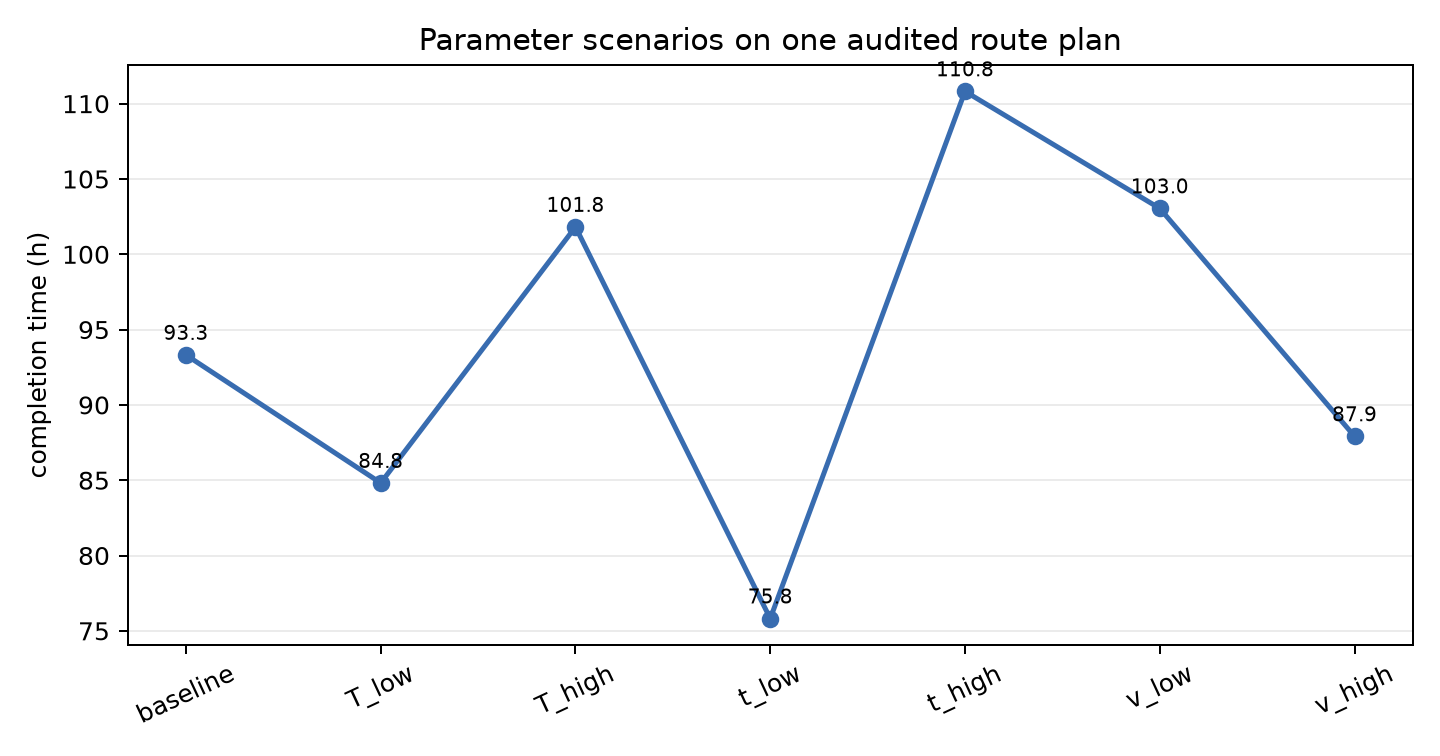
\includegraphics[width=0.82\linewidth]{figures/sensitivity_completion_time.png}
    \caption{同一路线结构在默认参数情景下的完成时间变化。}
    \label{fig:sensitivity-completion-time}
\end{figure}

从该样例可见，村停留时间增大和车速降低会明显提高完成时间。
这符合公式~\eqref{eq:route-time} 的结构。
当路线中村节点较多时，$t$ 的变化直接放大停留负载。
当 $v$ 降低时，长路线的行驶时间占比上升，空间邻近性的重要性随之提高。

%==========================================================================
\section{技术细节与结果可视化}
%==========================================================================

\subsection{计算实现说明}

计算程序围绕三个核心步骤展开。
首先读取道路网络并构造必访节点之间的最短路闭包。
然后在闭包上评价候选路线，复算每条路线的行驶距离、停留时间和完成时间。
最后对候选方案进行覆盖、路径和指标一致性检查。
这种处理方式使路线构造和结果复核保持同一套数学口径。

交互界面只负责参数输入、算法调用、候选展示和动画播放。
所有距离、耗时和审计结论均来自上述计算模型。
图~\ref{fig:gui-overview} 展示了当前交互界面。

\begin{figure}[H]
    \centering
    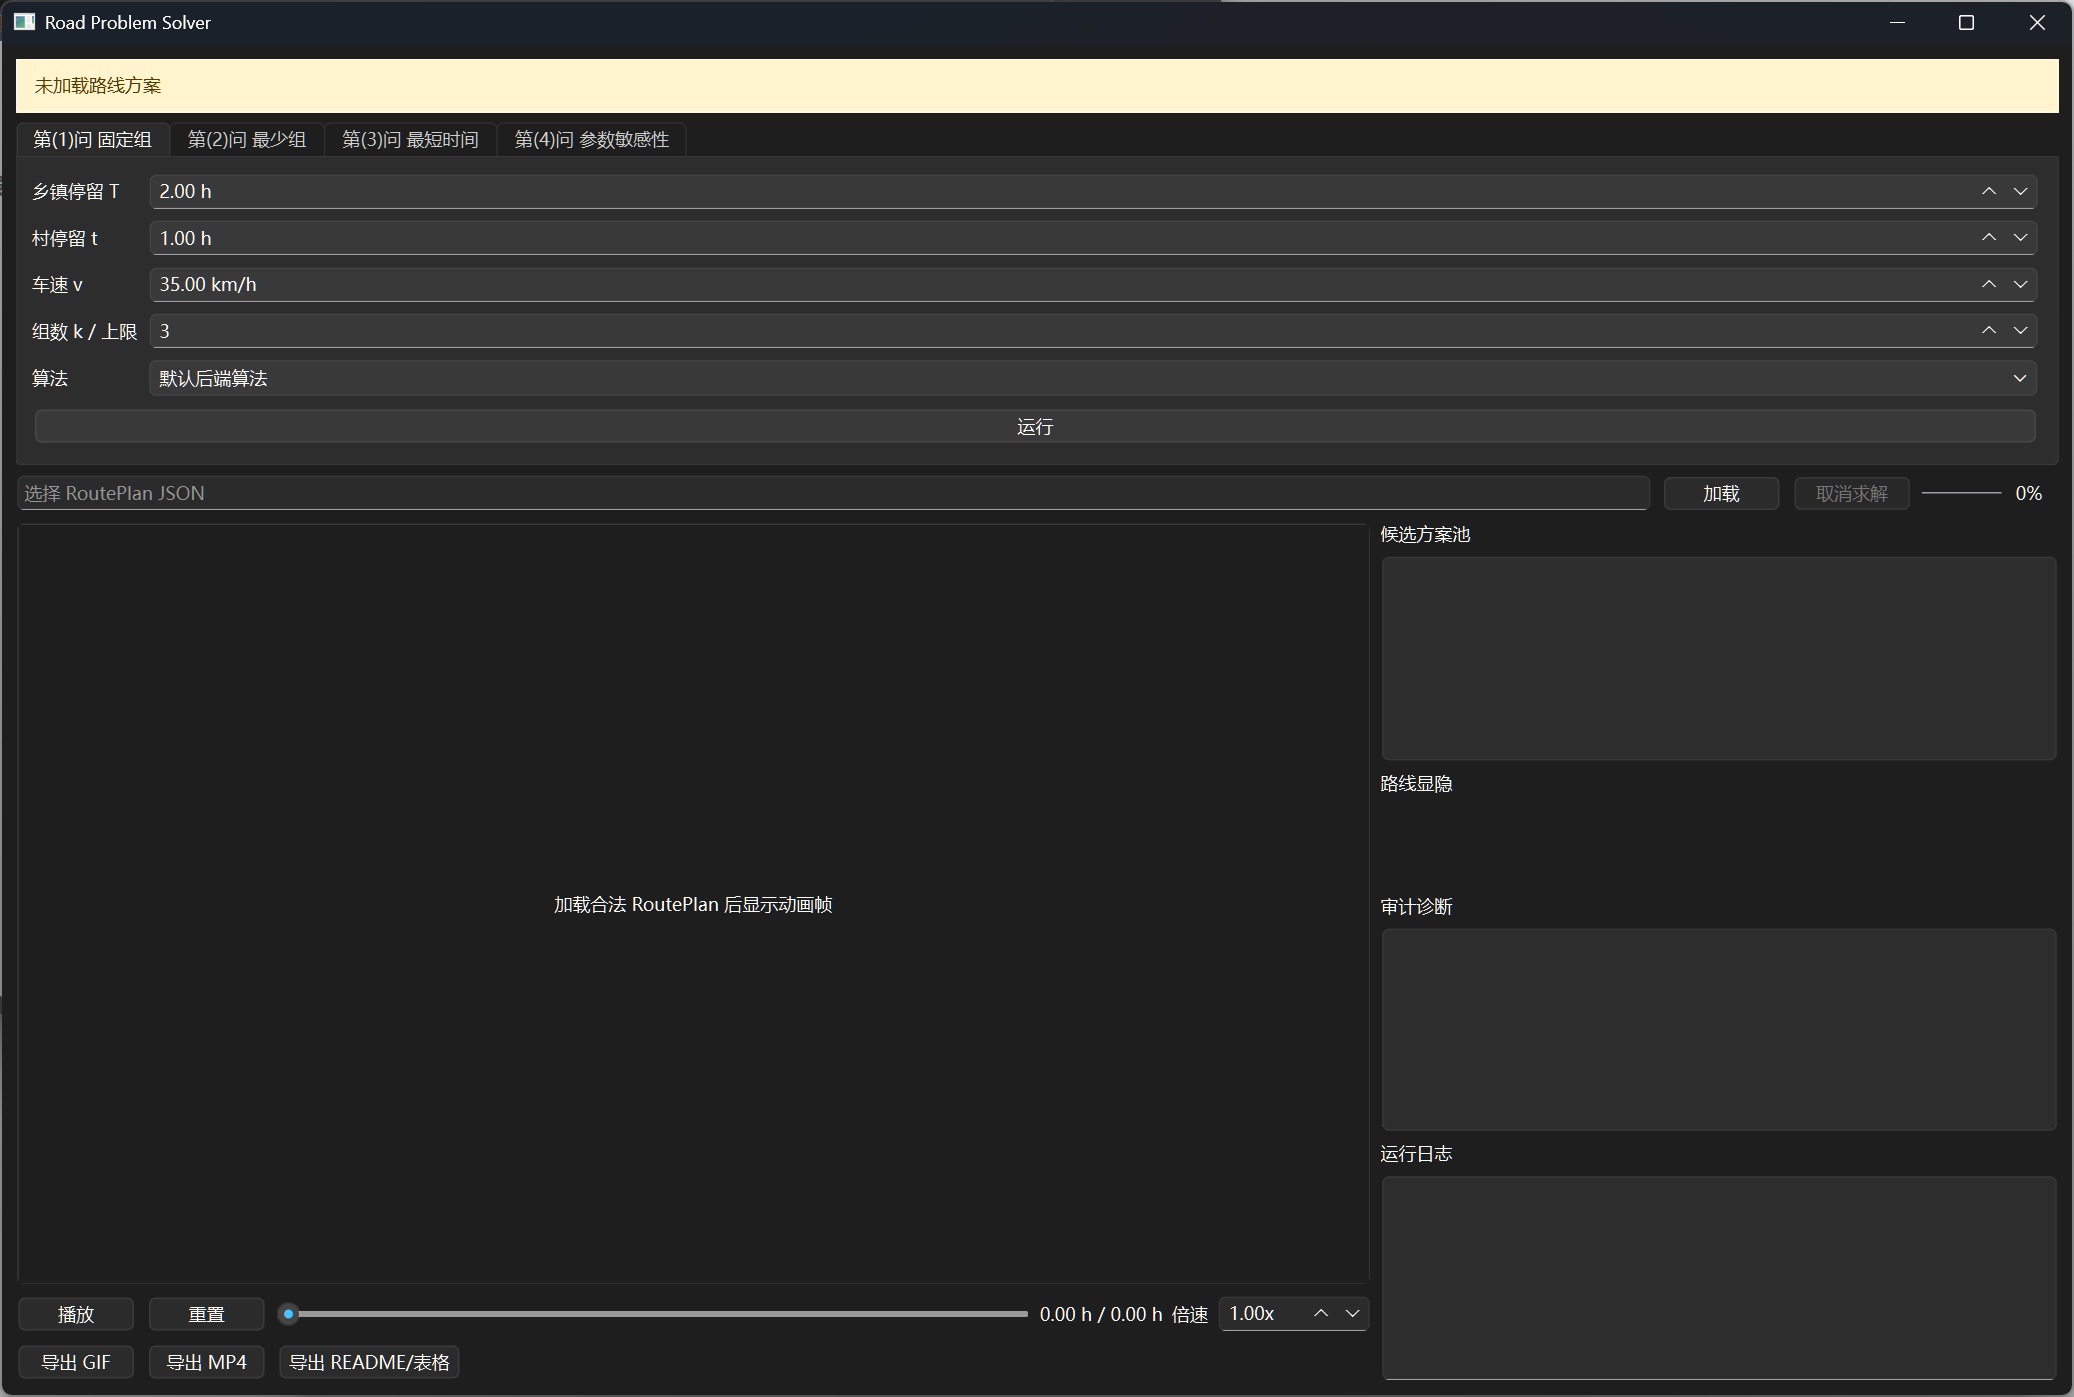
\includegraphics[width=0.94\linewidth]{figures/gui_overview.png}
    \caption{路线规划交互界面。界面按四个问题组织参数输入、求解入口、路线动画和审计诊断。}
    \label{fig:gui-overview}
\end{figure}

\subsection{路线动画时间轴}

可视化层把每条路线拆成行驶片段和停留片段。
边长为 $W$、车速为 $v$ 时，该边行驶时间为
\begin{equation}
    \tau = W/v.
\end{equation}
在地图布局中，若两端点的欧氏距离为 $d_{\text{map}}$，则地图上的移动速度为
\begin{equation}
    \frac{d_{\text{map}}}{\tau}
    =
    v\frac{d_{\text{map}}}{W}.
\end{equation}
这保证车辆在每条边上连续移动。
停留时，车辆保持在乡镇或村节点。
完成路线后，车辆回到 $O$ 并保持可见。

图形界面还可导出 GIF 或 MP4，用于展示巡视队伍沿路线连续移动的过程。
本文仍以静态图为主，动画文件作为展示附件。

%==========================================================================
\section{实验样例与结果分析}
%==========================================================================

\subsection{实验环境与数据}

当前实验使用正式道路网络文件 \texttt{data/raw/road\_network.tsv}。
道路网络读取结果无错误。
路网规模见表~\ref{tab:network-statistics}。

\begin{table}[H]
    \centering
    \caption{正式道路网络规模}
    \label{tab:network-statistics}
    \begin{tabular}{lr}
        \toprule
        项目 & 数量 \\
        \midrule
        总节点数 & 59 \\
        无向边数 & 94 \\
        乡镇节点数 & 17 \\
        村节点数 & 35 \\
        辅助道路节点数 & 6 \\
        必访节点数 & 52 \\
        \bottomrule
    \end{tabular}
\end{table}


\subsection{路线求解结果}

图~\ref{fig:problem1-routes}--图~\ref{fig:problem3-routes} 展示了三个主要问题的界面求解结果。
图中彩色线路对应不同巡视组，右侧给出候选方案和最终审计状态。
后续若导出路线汇总表，可在图注中继续补入总路程、最长路线距离、距离极差和耗时极差等指标。

\begin{figure}[H]
    \centering
    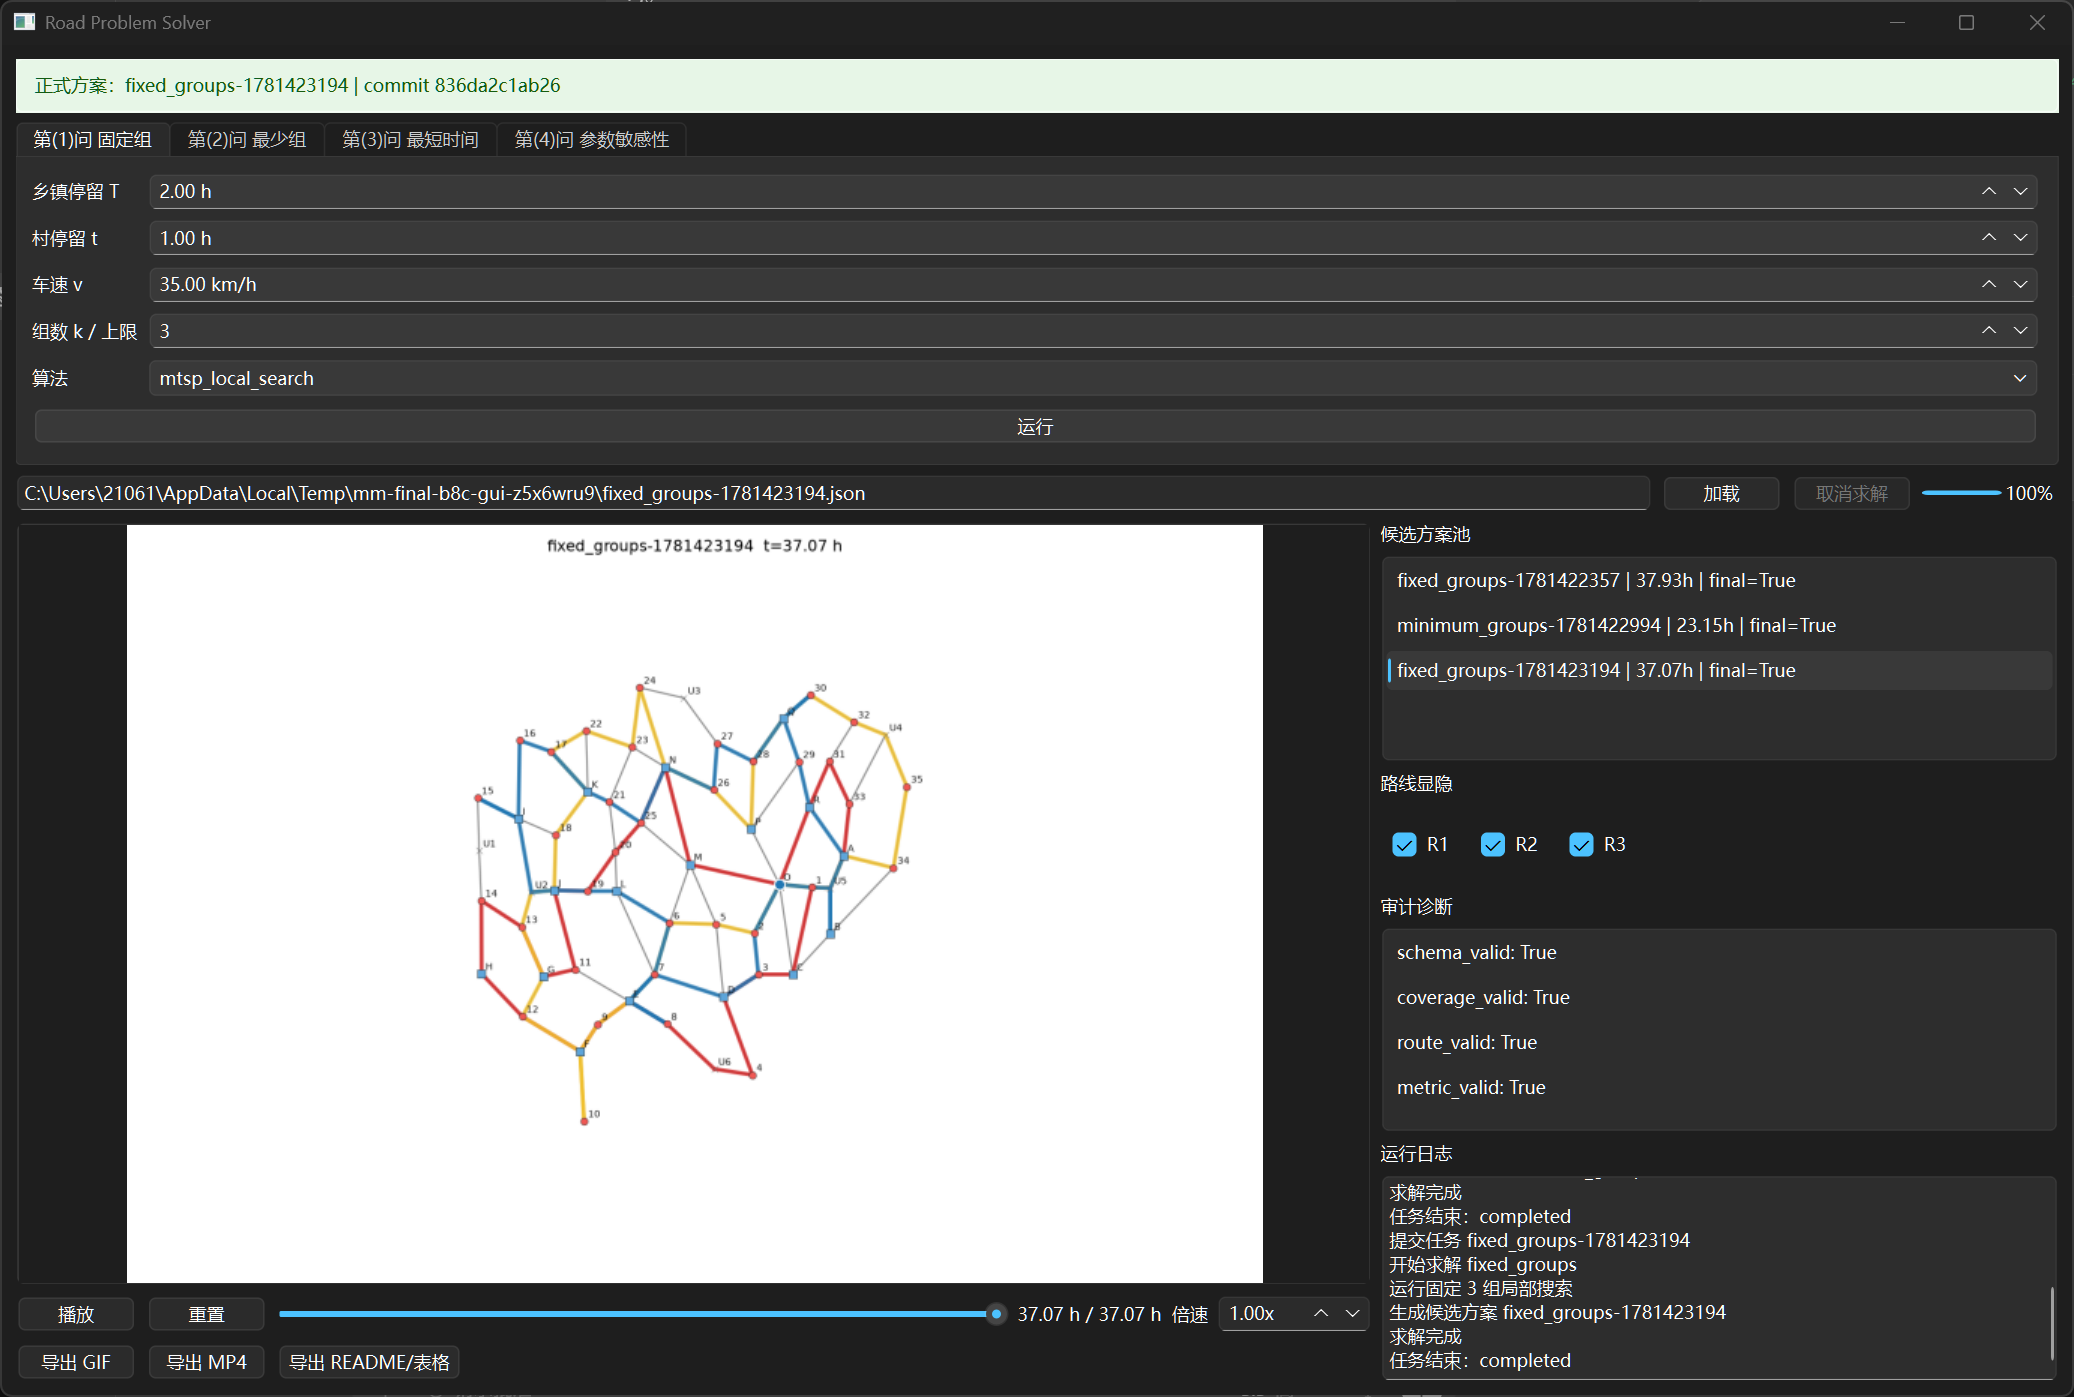
\includegraphics[width=0.94\linewidth]{figures/problem1_routes.png}
    \caption{第 (1) 问固定 $3$ 组的路线求解结果。该候选方案完成时间为 $37.07$ h，并通过最终审计。}
    \label{fig:problem1-routes}
\end{figure}

\begin{figure}[H]
    \centering
    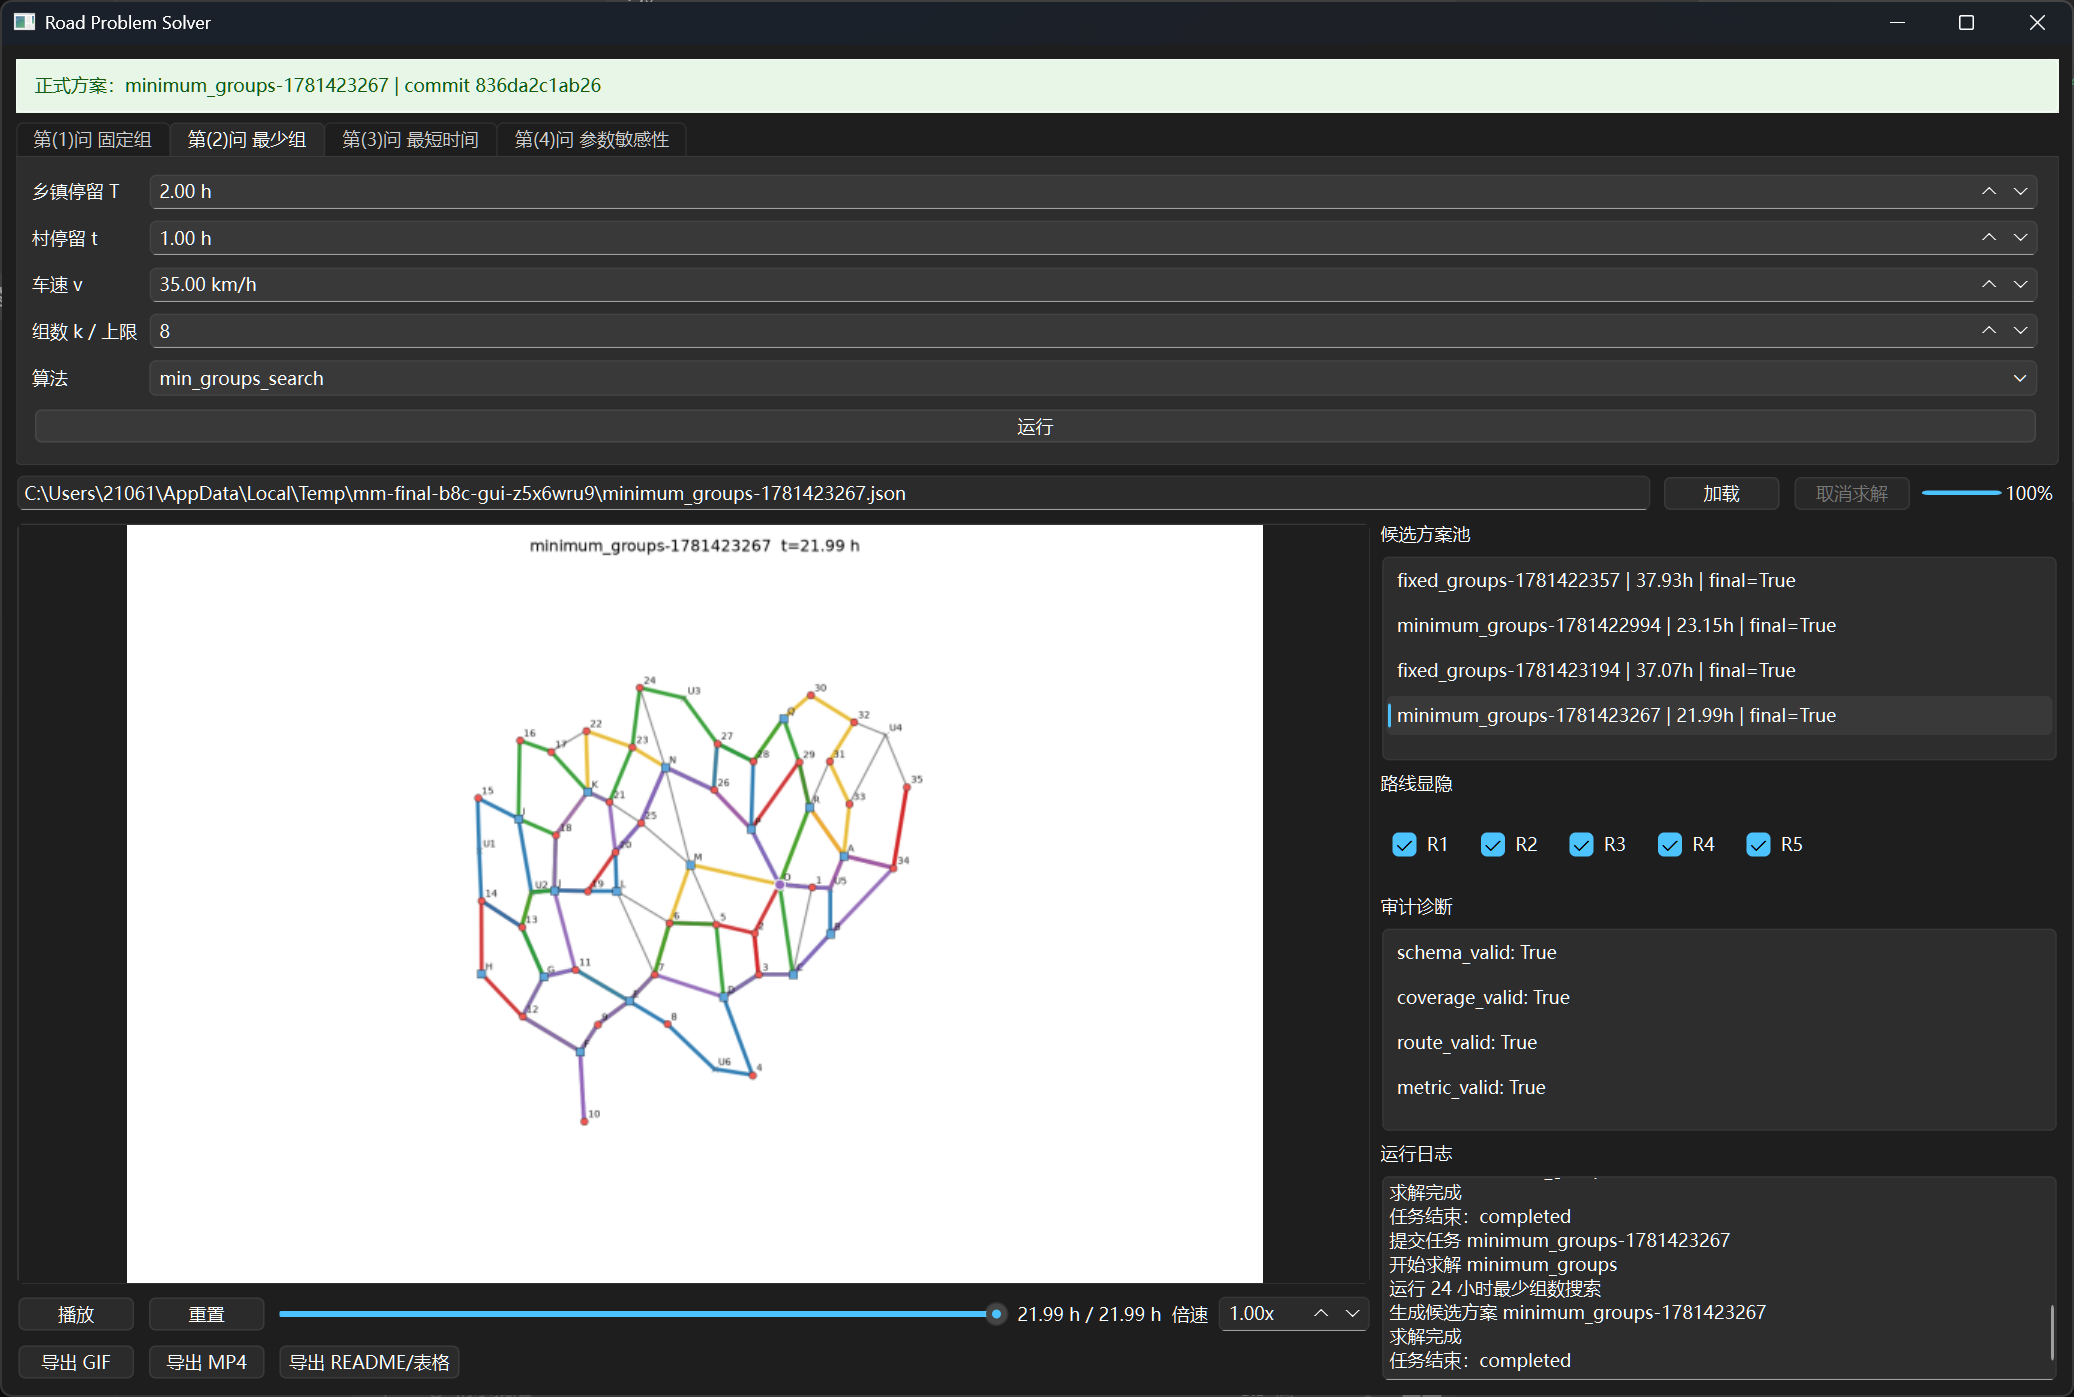
\includegraphics[width=0.94\linewidth]{figures/problem2_routes.png}
    \caption{第 (2) 问 $24$ 小时限制下的最少组数求解结果。该界面结果使用 $5$ 组，完成时间为 $21.99$ h，并通过最终审计。}
    \label{fig:problem2-routes}
\end{figure}

\begin{figure}[H]
    \centering
    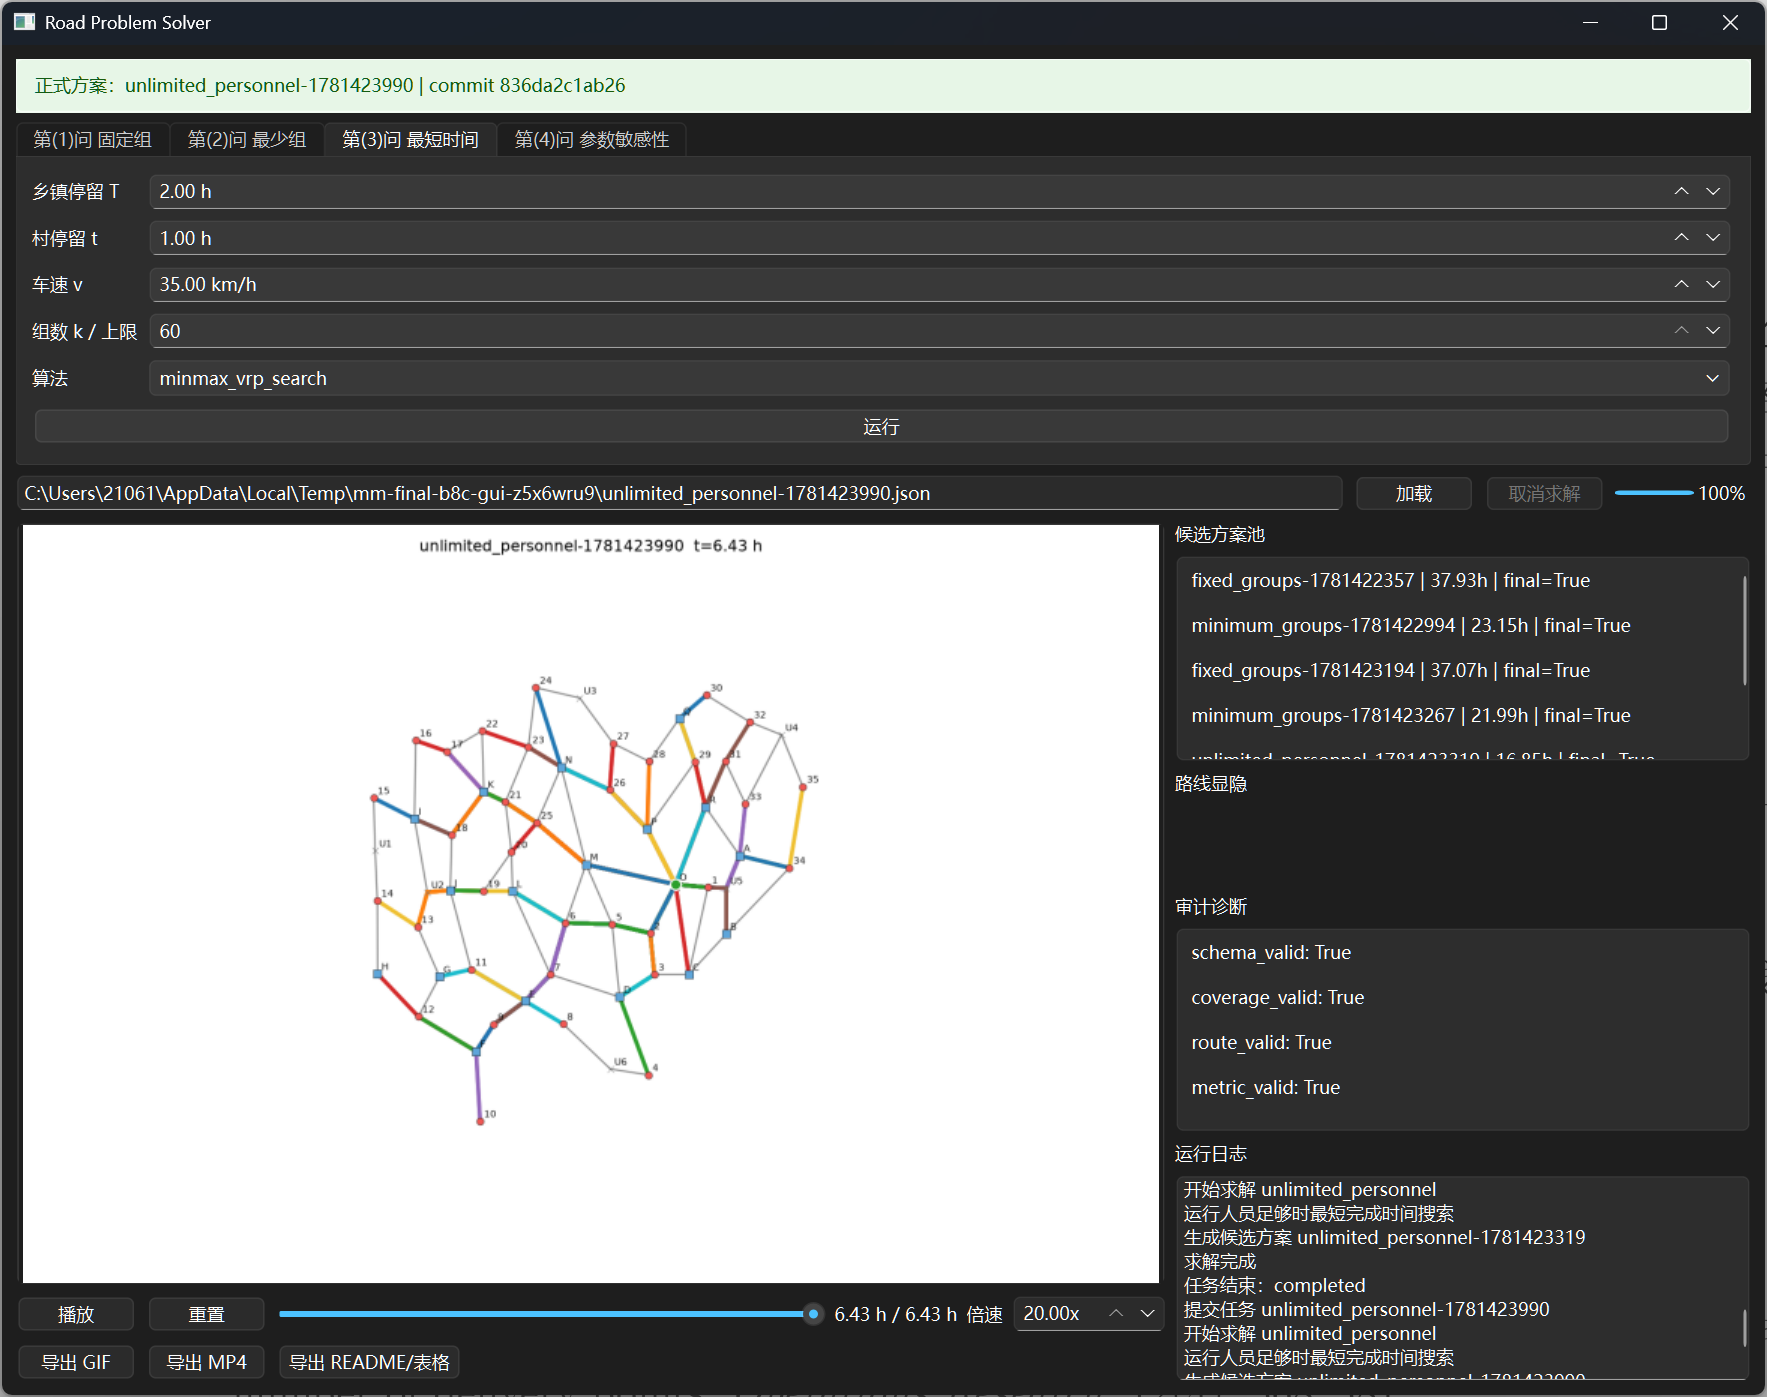
\includegraphics[width=0.94\linewidth]{figures/problem3_routes.png}
    \caption{第 (3) 问在人员足够时的最短完成时间求解结果。该界面将组数上限设为 $60$，求得完成时间为 $6.43$ h，与单点往返下界一致，并通过最终审计。}
    \label{fig:problem3-routes}
\end{figure}

\subsection{参数敏感性样例}

表~\ref{tab:sensitivity-sample} 展示同一路线结构在默认参数情景下的完成时间。

\begin{table}[H]
    \centering
    \caption{参数情景复算结果示例}
    \label{tab:sensitivity-sample}
    \begin{tabular}{lrrr}
        \toprule
        情景 & $T$ / h & $t$ / h & 完成时间 / h \\
        \midrule
        baseline & 2.0 & 1.0 & 93.32 \\
        T\_low & 1.5 & 1.0 & 84.82 \\
        T\_high & 2.5 & 1.0 & 101.82 \\
        t\_low & 2.0 & 0.5 & 75.82 \\
        t\_high & 2.0 & 1.5 & 110.82 \\
        v\_low & 2.0 & 1.0 & 103.04 \\
        v\_high & 2.0 & 1.0 & 87.91 \\
        \bottomrule
    \end{tabular}
\end{table}

该样例的结构很单纯，所以瓶颈路线始终为唯一路线。
即便如此，它仍清楚展示了参数影响方向。
$t$ 增大时，村节点服务时间成为主要增量来源。
$v$ 降低时，行驶时间被放大。
最终优化路线完成后，应使用多候选方案池重复这一分析，并比较候选赢家和瓶颈路线是否发生切换。

\placeholderfigure{此处放置最终参数敏感性热力图或折线图。建议横轴为参数情景，纵轴为完成时间，颜色区分候选路线，并标注需要重新优化的情景。}{第 (4) 问参数敏感性最终图占位}

%==========================================================================
\section{结论}
%==========================================================================

本文完成了县域巡视问题的统一图模型和审计分析框架。
模型把题面道路网络转化为无向加权图，把乡镇和村作为必须巡视节点，把辅助道路节点保留在通行路径中。
路线耗时由行驶时间、乡镇停留时间和村停留时间组成。
全方案完成时间取所有巡视组中的最大耗时。

当前可确认的结论包括：
\begin{enumerate}[leftmargin=2em]
    \item 默认参数下，总停留时间为 $69$ 小时，因此 $1$ 组和 $2$ 组均无法在 $24$ 小时内完成；
    \item 人员足够时，单点往返下界由节点 $H$ 给出，最短完成时间为约 $6.43$ 小时，单点一组证书可达到该下界；
    \item 参数敏感性分析应区分候选池最优和数学最优，当前实现会在候选排名、瓶颈路线或耗时结构明显变化时提示重新优化。
\end{enumerate}



\begin{thebibliography}{99}

\bibitem{clarke1964}
Clarke, G., \& Wright, J. W. (1964).
Scheduling of vehicles from a central depot to a number of delivery points.
\textit{Operations Research}, 12(4), 568--581.

\bibitem{kirkpatrick1983}
Kirkpatrick, S., Gelatt, C. D., \& Vecchi, M. P. (1983).
Optimization by simulated annealing.
\textit{Science}, 220(4598), 671--680.

\bibitem{tan2019}
谭永基，蔡志杰.
数学模型（第三版）.
上海：复旦大学出版社，2019.
ISBN 978-7-309-14289-1.

\end{thebibliography}

\end{document}
